\chapter{Complessità computazionale}
\section{Introduzione}
Fino ad adesso abbiamo studiato la teoria della calcolabilità, dato un problema abbiamo cercato di risolverlo 
tramite un modello computazionale (automi, macchine di Turing ecc...). Ci siamo concentrati solo sulla soluzione 
ma mai sulla complessità computazionale di tali soluzioni. In questo capitolo ci occuperemo proprio di questo e cercheremo di 
risolvere problemi tenendo conto sia della calcolabilità sia della complessità computazionale.
Le risorse che dobbiamo tenere in considerazione nello studio della complessità sono:
\begin{itemize}
    \item \textbf{Tempo}: quanto tempo impiega una macchina per risolvere il problema, infatti anche se una
    funzione è Turing calcolabile, se la macchina che la calcola ha bisogno di mesi, anni o secoli per terminare, la calcolabilità diventa inutile.

    \item \textbf{Spazio}: quanta memoria utilizza la macchina per risolvere il problema. Analogamente a quanto detto 
    per il tempo, se una funzione è Turing calcolabile ma necessita di miliardi di terabyte di memoria, la calcolabilità diventa inutile.
\end{itemize}
Un altro criterio importante per valutare la complessità è l'\textbf{input} di un problema. Intuitivamente
più l'input è grande e maggiore sarà la complessità, infatti per problemi reali una macchina di Turing 
deve sicuramente controllare tutto (o quasi) l'input prima di decidere di accettare. Ovviamente nell'analisi della
complessità dobbiamo sempre considerare il \textbf{caso peggiore}, quindi per ogni possibile dimensione $n \in \mathbb{N}$
dell'input, valuteremo l'input di dimensione $n$ che dà vita al consumo di risorse maggiore.\\
Ora vediamo in che modo calcoliamo la complessità temporale e spaziale:
\begin{itemize}
    \item Per la \textbf{risorsa tempo} impiegata da una macchina di Turing $M$ assumiamo che \textbf{ogni} \textbf{cambio di configurazione di } $\bm{M}$
    costi 1 unità. Definiamo una funzione matematica:
    \[    t_M : \mathbb{N} \to \mathbb{N}   \]
    che, per ogni $n \in \mathbb{N}$ restituisce il numero di configurazioni che la macchina deve attraversare prima 
    di terminare l'input di dimensione $n$. Il costo sarà quindi l'andamento asintotico di tale funzione $t_M$
    
    \item Per la \textbf{risorsa spazio} impiegata da una macchina di Turing $M$ assumiamo che \textbf{ogni cella di nastro di} $\bm{M}$.
    Definiamo una funzione matematica:
    \[  s_M : \mathbb{N} \to \mathbb{N}   \]
    che, per ogni $n \in \mathbb{N}$ restituisce il massimo numero di celle utilizzate dalla macchina durante una esecuzione per un input di dimensione $n$
    nello stesso istante di tempo (?). Il costo sarà l'andamento asintotico di tale funzione $s_M$ 
\end{itemize} 
Ovviamente l'andamento asintotico non fornisce una soluzione precisa ma ci dà comunque una indicazione di quanto tempo e spazio impieghi la macchina.
\newpage
\subsection{Andamento asintotico e Notazione O-grande}
Per descrivere il comportamento asintotico di una funzione utlizziamo la notazione O-grande:\smallskip\\
\colorbox{SALZO}{\parbox{\dimexpr\linewidth-2\fboxsep}{\begin{definition}
   Siano $f:\mathbb{N}\to \mathbb{N}$ e $g:\mathbb{N}\to \mathbb{N}$ due funzioni. $f(n)$ è un \textbf{O-grande} di $g(n)$
   \[   f(n) = \mathcal{O}\big( g(n)  \big)   \]
   se esistono due costanti $c > 0 $ e $n_0 \ge 0$ tali che:
   \[    f(n) \le c \cdot g(n), \qquad \text{per ogni } n \ge n_0  \]
\end{definition}}}\smallskip\\
In altre parole $f(n)$ cresce al più quanto $g(n)$, a partire da un certo valore di $n \ (n_0)$. Graficamente:
\begin{figure}[H]
    \centering  
    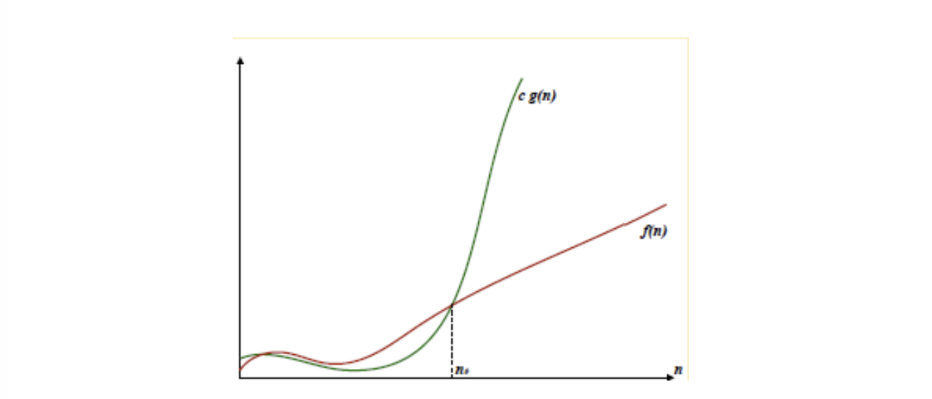
\includegraphics[width=0.7\linewidth]{../../images/ogra.png}
    %\caption{caption}
    %\label{label}
\end{figure}   
\noindent Dall'immagine è chiaro che dopo $n_0$ il valore di $f(n)$ è più piccolo di $c \cdot g(n)$.\\
Ecco alcune \textbf{proprietà} sull'andamento asintotico:
\begin{itemize}[label = --]
    \item L'andamento asintotico di una somma dipende dal termine più "veloce" (dominante)
    \[   f(n) + g(n) = \mathcal{O} \big(\max \{ f(n),g(n)  \}     \big)   \]
    \item L'andamento asintotico di un prodotto dipende da entrambi gli operandi
    \[ \text{Se }f(n) = \mathcal{O}(h) \text{ e } g(n) = \mathcal{O}(k) \text{ allora } f(n) \cdot g(n) = \mathcal{O}\big( h(n) \cdot k(n)   \big)   \]
    \item L'andamento asintotico è transitivo
    \[   \text{Se } f(n) = \mathcal{O}\big( g(n)  \big) \text{ e } g(n) = \mathcal{O} \big( h(n) \big) \text{ allora } f(n) = \mathcal{O}\big( h(n) \big) \]
\end{itemize}
Ora vediamo alcuni \textbf{andamenti asintotici} \textbf{noti}:
\begin{itemize}
    \item \textbf{Costanti}: funzioni costanti non crescono al variare di $n$. Per ogni costante $c$:
    \[  c = \mathcal{O}\big(  g(n) \big), \quad \text{per ogni } g(n) \text{ limitata inferiormente da } c \in \mathbb{N}   \]

    \item \textbf{Polinomi}: un polinomio cresce asintoticamente come il suo termine di grado maggiore. Sia 
    \[ p(n) =  c_0 + c_1 n^1 + ... + c_n n^m  \]
    un polinomio di grado $m$, quindi avrò che:
    \[    p(n) = \mathcal{O}(n^m)  \]
    
    \item \textbf{Logaritmi}: il logaritmo scresce asintoticamente meno di un polinomio. Sia $p(n)$ un polinomio di grado almeno 1. Si ha che:
    \[    \log(n) = \mathcal{O}\big(  p(n)  \big)   \]

    \item \textbf{Esponenziali}: un polinomio cresce asintoticamente meno di un esponenziale. Sia $p(n)$ un polinomio. Si ha che:
    \[  p(n) = \mathcal{O} (t^n), \quad \text{per ogni } t > 1  \]

\end{itemize}




\section{Complessità temporale Deterministica}
Sia $M = < \Sigma , \Gamma, Q, \delta, q_0,q_{yes}, q_{no}>$ una macchina di Turing e $x$ un input per $M$.
Per definire la complessità temporale deterministica utilizzeremo la notazione $\bm{E_M(x)}$ per indicare l'unica \textbf{esecuzione} di $M$ su $x$.\smallskip\\
\colorbox{SALZO}{\parbox{\dimexpr\linewidth-2\fboxsep}{\begin{definition}
   La \textbf{complessità temporale} $t_m: \mathbb{N}\to \mathbb{N}$ di $M$ è la funzione
   \[  t_M (n) = \max_{\{x \in \Sigma^* | \ |x| = n\}} |E_M(x)|   \]
\end{definition}}}\smallskip\\

